%!TEX program = xelatex
\documentclass[8pt, landscape, a4paper]{extarticle}

% --- 核心宏包 ---
\usepackage[UTF8, fontset=fandol]{ctex}
\usepackage[margin=0.8cm, top=1cm, bottom=1.3cm]{geometry}
\usepackage{multicol}
\usepackage{xcolor}
\usepackage{tcolorbox}
\usepackage{enumitem}
\usepackage{amsmath}
\usepackage{amssymb}
\usepackage{fontspec}
\usepackage{tikz}
\usetikzlibrary{arrows.meta, shapes}

% --- 去掉页码 ---
\pagestyle{empty}

% --- 颜色定义 (棕色/铜色主题) ---
\definecolor{headerblue}{RGB}{160, 82, 45}     % Sienna (土黄/棕)
\definecolor{navcolor}{RGB}{211, 84, 0}        % 导航橙
\definecolor{intuitioncolor}{RGB}{41, 128, 185}% 直觉蓝
\definecolor{accentcolor}{RGB}{192, 57, 43}    % 强调红
\definecolor{section2}{RGB}{142, 68, 173}      % 紫色
\definecolor{dividergray}{RGB}{220, 220, 220}

% --- 全局设置 ---
\setlength{\parindent}{0pt}
\setlength{\columnsep}{0.4cm} 
\linespread{1.1} 

% --- 列表样式 ---
\setlist[itemize]{leftmargin=1.2em, nosep, itemsep=2pt, topsep=2pt, label=$\textcolor{headerblue}{\vcenter{\hbox{\tiny$\bullet$}}}$ }
\setlist[description]{leftmargin=0.2em, style=sameline, nosep, itemsep=2pt, font=\bfseries}

% --- Box 样式 ---
\newtcolorbox{mybox}[2][]{%
  colback=white,
  colframe=#2,
  coltitle=white,
  boxrule=1pt,             
  arc=2mm,                 
  left=4pt, right=4pt, top=3pt, bottom=3pt, 
  toptitle=3pt, bottomtitle=3pt, 
  fonttitle=\bfseries\sffamily\large,
  title={#1},
  after skip=5pt          
}

% --- 自定义命令 ---
\newcommand{\subt}[1]{{\vspace{2pt}\textbf{\large \textcolor{black}{#1}}}}

\newcommand{\boxdesc}[1]{%
    \textit{\small \textcolor{gray}{#1}}%
    \par\vspace{2pt}%
    {\color{dividergray}\hrule height 0.5pt}%
    \vspace{2pt}%
}

\newcommand{\sepline}{%
    \par \vspace{3pt}%
    {\color{dividergray}\hrule height 0.5pt}%
    \par \vspace{3pt}%
}

% 公式间距
\setlength{\abovedisplayskip}{3pt}
\setlength{\belowdisplayskip}{3pt}

\begin{document}

% --- 页眉 ---
\begin{center}
    {\Huge \textbf{\sffamily \textcolor{headerblue}{凸优化 Convex Optimization Cheat Sheet}}} \\
    \vspace{0.2cm}
    {\large \texttt{The Science of Best Choices: From Gradient Descent to Duality}}
\end{center}

% --- 开始四栏布局 ---
\begin{multicols*}{4}

% === 第一栏 ===

\begin{mybox}[️ 场景导航 (Use Cases)]{navcolor}
    \boxdesc{遇到什么问题 $\to$ 用什么工具}
    \begin{itemize}[itemsep=2pt]
        \item \textbf{模型训练/拟合} $\to$ 梯度下降 (SGD / Adam)
        \item \textbf{资源分配/调度} $\to$ 线性规划 (LP)
        \item \textbf{稀疏解/特征选择} $\to$ Lasso ($L_1$ 正则)
        \item \textbf{投资组合优化} $\to$ 二次规划 (QP)
        \item \textbf{约束满足问题} $\to$ 拉格朗日乘子法
        \item \textbf{超大规模求解} $\to$ ADMM
    \end{itemize}
\end{mybox}

\begin{mybox}[1. 凸性基础 (Convexity)]{headerblue}
    \boxdesc{碗状世界,绝无局部陷阱}
    
    \subt{凸集 (Convex Set)}
    集合内任意两点的连线仍在集合内。
    $$ \theta x + (1-\theta)y \in C, \quad \forall \theta \in [0,1] $$
    \sepline
    
    \subt{凸函数 (Convex Function)}
    函数图像上方的区域是凸集 (弦在弧之上)。
    $$ f(\theta x + (1-\theta)y) \le \theta f(x) + (1-\theta)f(y) $$
    \begin{itemize}
        \item \textbf{一阶条件}: $f(y) \ge f(x) + \nabla f(x)^T(y-x)$ (切线在下)。
        \item \textbf{二阶条件}: $\nabla^2 f(x) \succeq 0$ (Hessian 半正定)。
    \end{itemize}
    \sepline
    
    \subt{核心性质}
    \textbf{局部最优 $\implies$ 全局最优}。
    \textit{这是凸优化最强大的保证。}
    \textbf{常见凸函数}: $e^x$, $x^2$, $-\log x$, $\|x\|_p$ ($p \ge 1$)。
\end{mybox}

\begin{mybox}[2. 标准形式 (Standard Form)]{headerblue}
    \boxdesc{把问题装进笼子}
    
    $$ \begin{aligned} 
    \min \quad & f_0(x) \\
    \text{s.t.} \quad & f_i(x) \le 0, \quad i=1,\dots,m \\
    & h_i(x) = 0, \quad i=1,\dots,p 
    \end{aligned} $$
    \begin{itemize}
        \item $f_0, f_i$ 必须是\textbf{凸函数}。
        \item $h_i$ 必须是\textbf{仿射函数} ($Ax+b$)。
    \end{itemize}
\end{mybox}

\columnbreak

% === 第二栏 ===

\begin{mybox}[3. 对偶理论 (Duality)]{headerblue}
    \boxdesc{从另一个角度看问题}
    
    \subt{拉格朗日函数 (Lagrangian)}
    把约束加权放到目标函数里:
    $$ L(x, \lambda, \nu) = f_0(x) + \sum \lambda_i f_i(x) + \sum \nu_i h_i(x) $$
    ($\lambda_i \ge 0$)
    \sepline
    
    \subt{对偶函数 (Dual Function)}
    $g(\lambda, \nu) = \inf_x L(x, \lambda, \nu)$。
    \begin{itemize}
        \item $g$ 永远是\textbf{凹函数} (即使原问题非凸)。
        \item \textbf{弱对偶}: $d^* \le p^*$ (下界)。
        \item \textbf{强对偶}: $d^* = p^*$ (Slater 条件满足时)。
    \end{itemize}
    \sepline
    
    \subt{KKT 条件 (KKT Conditions)}
    \textbf{最优解的必要条件} (强对偶下也是充分条件):
    \begin{enumerate}
        \item \textbf{平稳性}: $\nabla_x L = 0$ (梯度为0)。
        \item \textbf{原始可行}: 满足原约束。
        \item \textbf{对偶可行}: $\lambda_i \ge 0$。
        \item \textbf{互补松弛}: $\lambda_i f_i(x) = 0$ (关键!)。
    \end{enumerate}
    \textit{直觉:要么约束没起作用 ($\lambda=0$),要么约束紧绷 ($f=0$)。}
\end{mybox}

\begin{mybox}[4. 典型问题类 (Classes)]{headerblue}
    \boxdesc{常见的优化模型}
    
    \subt{线性规划 (LP)}
    目标和约束都是线性的。
    \textit{解法: 单纯形法 (Simplex), 内点法。}
    \sepline
    
    \subt{二次规划 (QP)}
    目标是二次的 ($x^TPx$),约束是线性的。
    \textit{场景: SVM, 最小二乘。}
    \sepline
    
    \subt{半定规划 (SDP)}
    变量是矩阵,约束是半正定 ($X \succeq 0$)。
    \textit{场景: 控制理论, 组合优化松弛。}
    \sepline
    
    \subt{锥优化 (Cone Programming)}
    约束是锥:$x \in K$(如二阶锥 SOC)。
    \textit{统一框架:LP, QP, SDP 都是特殊情况。}
\end{mybox}

\columnbreak

% === 第三栏 ===

\begin{mybox}[5. 求解算法 (Algorithms)]{headerblue}
    \boxdesc{如何一步步走到山谷}
    
    \subt{梯度下降 (Gradient Descent)}
    $$ x_{k+1} = x_k - \alpha \nabla f(x_k) $$
    \begin{itemize}
        \item \textbf{SGD}: 每次只用一个样本算梯度 (快但抖)。
        \item \textbf{Momentum}: 加惯性,冲过鞍点。
    \end{itemize}
    \sepline
    
    \subt{牛顿法 (Newton's Method)}
    利用二阶信息 (Hessian) 调整方向和步长。
    $$ x_{k+1} = x_k - [\nabla^2 f(x_k)]^{-1} \nabla f(x_k) $$
    \textit{收敛极快 (二次收敛),但求逆矩阵贵 ($O(n^3)$)。}
    \sepline
    
    \subt{拟牛顿法 (BFGS)}
    近似 Hessian 矩阵,避免求逆。
\end{mybox}

\begin{mybox}[6. 正则化与稀疏 (Regularization)]{headerblue}
    \boxdesc{奥卡姆剃刀:简单即美}
    
    \subt{L2 正则 (Ridge)}
    $\min \|Ax-b\|^2 + \lambda \|x\|_2^2$
    \begin{itemize}
        \item 防止过拟合,权重平滑。
        \item 对应高斯先验。
    \end{itemize}
    \sepline
    
    \subt{L1 正则 (Lasso)}
    $\min \|Ax-b\|^2 + \lambda \|x\|_1$
    \begin{itemize}
        \item \textbf{稀疏性}: 产生大量为 0 的系数。
        \item \textbf{几何直觉}: $L_1$ 球是有棱角的 (菱形),等高线容易碰到角 (坐标轴)。
        \item 对应拉普拉斯先验。
    \end{itemize}
\end{mybox}

\begin{mybox}[7. Python / CVXPY 实战]{headerblue}
    \boxdesc{声明式编程求解}
    \begin{itemize}
        \item \texttt{x = cp.Variable(n)}
        \item \texttt{prob = cp.Problem(cp.Minimize(obj), [constraints])}
        \item \texttt{prob.solve()}
        \item \textbf{Scipy}: \texttt{minimize(fun, x0, method='BFGS')}
    \end{itemize}
\end{mybox}

\columnbreak

% === 第四栏 ===

\begin{mybox}[8. 高阶技巧 (Tricks)]{headerblue}
    \boxdesc{化腐朽为神奇}
    
    \subt{松弛 (Relaxation)}
    把难解的非凸问题 (如整数规划) 放宽为凸问题 (如 LP),求下界。
    \sepline
    
    \subt{坐标下降 (Coordinate Descent)}
    每次只优化一个变量,固定其他。
    \textit{适合 Lasso 等非光滑问题。}
    \sepline
    
    \subt{ADMM}
    交替方向乘子法。将大问题拆分为小问题分布式求解。
    \sepline
    
    \subt{投影梯度法 (Projected Gradient)}
    处理约束:$x_{k+1} = \Pi_C(x_k - \alpha \nabla f(x_k))$。
    \textit{$\Pi_C$ 将点投影回可行域 $C$。}
\end{mybox}

\vspace*{\fill}

\begin{mybox}[ 核心直觉 (Intuition)]{intuitioncolor}
    \boxdesc{“万物皆可优化。”}
    
    % TikZ 矢量图: 展示凸函数与梯度下降,或者 L1 vs L2
    \begin{center}
    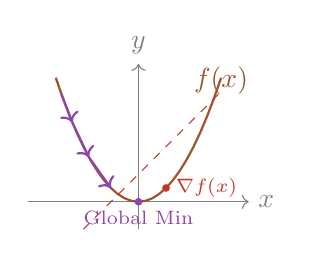
\begin{tikzpicture}[scale=0.7]
        % 坐标轴
        \draw[->, gray] (-2,0) -- (2,0) node[right] {$x$};
        \draw[->, gray] (0,-0.5) -- (0,2.5) node[above] {$y$};
        
        % 凸函数抛物线
        \draw[thick, headerblue, domain=-1.5:1.5] plot (\x, {\x*\x});
        \node[headerblue] at (1.5, 2.2) {$f(x)$};
        
        % 切线 (支持平面)
        \draw[dashed, accentcolor] (-1, -0.5) -- (1.5, 2);
        \fill[accentcolor] (0.5, 0.25) circle (2pt);
        \node[right, accentcolor, font=\scriptsize] at (0.5, 0.25) {$\nabla f(x)$};
        
        % 全局最小值
        \fill[section2] (0,0) circle (2pt);
        \node[below, section2, font=\scriptsize] at (0,0) {Global Min};
        
        % 梯度下降箭头
        \draw[->, thick, section2] (-1.4, 1.96) -- (-1.2, 1.44);
        \draw[->, thick, section2] (-1.2, 1.44) -- (-0.9, 0.81);
        \draw[->, thick, section2] (-0.9, 0.81) -- (-0.5, 0.25);
    \end{tikzpicture}
    \end{center}

    \hspace{1em}凸优化的美妙之处在于\textbf{确定性}。如果你能把工程问题建模为凸问题,那么你一定能找到最优解,而且很快。
    \vspace{4pt}
    
    \subt{三大核心视角}
    \begin{itemize}[itemsep=4pt]
        \item \textbf{梯度即方向}: 
        在黑暗的山脉中,梯度是唯一的指路明灯,告诉我们往哪里走下降最快。
        
        \item \textbf{对偶即定价}: 
        拉格朗日乘子 $\lambda$ 不仅仅是数学辅助量,它是资源的\textbf{影子价格}。如果约束放松一点,目标函数能优化多少?$\lambda$ 告诉你答案。
        
        \item \textbf{稀疏即选择}: 
        $L_1$ 正则化不仅仅是数学技巧,它是一种哲学:在纷繁复杂的因素中,只有少数几个是关键的 (Occam's Razor)。
    \end{itemize}
    
    \vspace{6pt}
    \centering\textit{\footnotesize 既然无法遍历所有可能,那就沿着梯度滑向谷底。}
\end{mybox}

\end{multicols*}

\end{document}
